% presentation
%\documentclass[compress,draft]{beamer}
\documentclass[compress,aspectratio=1610]{beamer}
%\documentclass[compress,aspectratio=1610,handout]{beamer}

\usepackage{../mtex,fancyvrb,booktabs,multirow,makecell}
\usepackage{tikz,pgfplots}
\usetikzlibrary{shapes}

%\usepackage{subfigure}
\usepackage[labelformat=empty]{subcaption}
\captionsetup{compatibility=false}
%\usepackage[inline]{enumitem}
\newcommand\paraitem{%
  \;
  \makebox[\labelwidth][r]{%
    \makelabel{%
      \usebeamertemplate{itemize \beameritemnestingprefix item}}}\hskip\labelsep}


\newcommand{\SO}{\mathrm{SO}(3)}
\newcommand{\rot}[1]{\mathbf{#1}}
\newcommand{\ds}{\displaystyle}
\newcommand{\R}{\mathbb R}
\renewcommand{\S}{\mathbb S}
\newcommand{\conj}[1]{\overline{#1}}
\newcommand{\norm}[1]{\lVert #1\rVert}
\newcommand{\abs}[1]{\lvert #1\rvert}

\usepackage{pifont}
\definecolor{darkgreen}{rgb}{0,0.7,0}      % hellgruener Rahmen
\definecolor{darkred}{rgb}{0.7,0,0}      % hellgruener Rahmen
\definecolor{darkyellow}{rgb}{0.8,0.65,0}      % hellgruener Rahmen
\newcommand{\checked}{\textcolor{darkgreen}{\ding{51}}}
\newcommand{\crossed}{\textcolor{darkred}{\ding{54}}}
\newcommand{\ok}{\textcolor{darkyellow}{\ding{108}}}

\newcommand{\mytriangle}[1]{\tikz{\node[draw=#1,fill=#1,isosceles
triangle,isosceles triangle stretches,shape border rotate=90,minimum
width=0.2cm,minimum height=0.2cm,inner sep=0pt] at (0,0) {};}}

\usetikzlibrary{fit}
% \tikzset{%
%   highlight/.style={rectangle,rounded corners,fill=red!15,draw,
%     fill opacity=0.5,thick,inner sep=0pt}
%   }
\tikzset{%
  highlight/.style={rectangle,rounded corners,draw,red,
    fill opacity=0.5,thick,inner sep=0pt}
}
% see https://tex.stackexchange.com/questions/40028/highlight-elements-in-the-matrix

\newcommand{\tikzmark}[2]{\tikz[overlay,remember picture,
  baseline=(#1.base)] \node (#1) {#2};}
%
\newcommand{\Highlight}[1][submatrix]{%
    \tikz[overlay,remember picture]{
    \node[highlight,fit=(left.north west) (right.south east)] (#1) {};}
}


\author{R. Hielscher}

\title{ODF Reconstruction from Pole Figure Data}

\institute{Faculty of Mathematics,\\
  TU Bergakademie Freiberg, Germany}

\date{MTEX Workshop 2024}

\newcommand{\crystal}[5]{%
  \draw[->, >=latex, #5] (#1) --+ (#2);%
  \draw[->, >=latex, #5] (#1) --+ (#3);%
  \draw[->, >=latex, #5] (#1) --+ (#4);%
}

\newcommand{\fillcrystal}[5]{%
  \filldraw[fill=red!25,draw=red!35,opacity=0.5]
%  (0,0) + (1,0) -- (0,0) --++ (0,1) --+ (1,0);
  (#1) +(#2) -- (#1) --++ (#3) -- +(#2) ;%
  \filldraw[fill=red!45,draw=red!35,opacity=0.5]
  (#1) +(#3) -- (#1) --++ (#4) -- +(#3) ;%
  \filldraw[fill=red!65,draw=red!35,opacity=0.5]
  (#1) +(#4) -- (#1) --++ (#2) -- +(#4) ;%
  \draw[->, >=latex, #5] (#1) --+ (#2);%
  \draw[->, >=latex, #5] (#1) --+ (#3);%
  \draw[->, >=latex, #5] (#1) --+ (#4);%
}

\newcommand{\filldirection}[5]{%
  \filldraw[fill=red!25,draw=red!35,opacity=0.5]
%  (0,0) + (1,0) -- (0,0) --++ (0,1) --+ (1,0);
  (#1) +(#2) -- (#1) --++ (#3) -- +(#2) ;%
  \filldraw[fill=red!45,draw=red!35,opacity=0.5]
  (#1) +(#3) -- (#1) --++ (#4) -- +(#3) ;%
  \filldraw[fill=red!65,draw=red!35,opacity=0.5]
  (#1) +(#4) -- (#1) --++ (#2) -- +(#4) ;%
  \draw[->, >=latex, #5] (#1) --+ (#2);%
  \draw[->, >=latex, #5] (#1) --+ (#3);%
  \draw[->, >=latex,color=red, very thick] (#1) --+ (#4);%
}


\begin{document}

\begin{frame}
  \maketitle{}
\end{frame}

% \begin{frame}
%   \frametitle{Table of Content}

% \tableofcontents{}

% \end{frame}


\begin{frame}
  \frametitle{Braggs Law}


  % \begin{itemize}
  % \item<+-> $\vec s = \vec s_{\text{out}}- \vec s_{\text{in}}$ is the bisector between
  %   $\vec s_{\text{out}}$ and $\vec s_{\text{in}}$ $\implies$ $\abs{\vec s} = 2 \sin \theta$
  % \item<+-> $\vec S = \frac{\vec s}{\lambda} = (h k \ell)$ is a lattice plane normal
  %   % $\implies$ $d_{h k \ell} = \frac{\gcd(h,k,\ell)}{\abs{\vec S}}
  %   % = \frac{\lambda \gcd(h,k,\ell)}{2 \sin \theta}$
  %    $\implies$ $\frac{2 \sin \theta}{\lambda} = \frac{1}{d_{h k \ell}}$
  % \end{itemize}

  \begin{itemize}
  \item $\lambda$ - wave length
  \item $2\theta$ - angle between beam source $\vec s_{\text{in}}$ and
    detector $\vec s_{\text{out}}$

  \item $d_{hk\ell} = 1/\norm{\{hk\ell\}}_{2}$ - distance between the lattice
    planes $\{hk\ell\}$
  \end{itemize}

  \begin{block}{}
    \begin{equation*}
      2 d_{hk\ell} \sin \theta = n \lambda, \quad n = 1,2,\ldots
    \end{equation*}
  \end{block}

  \begin{figure}
  \centering
  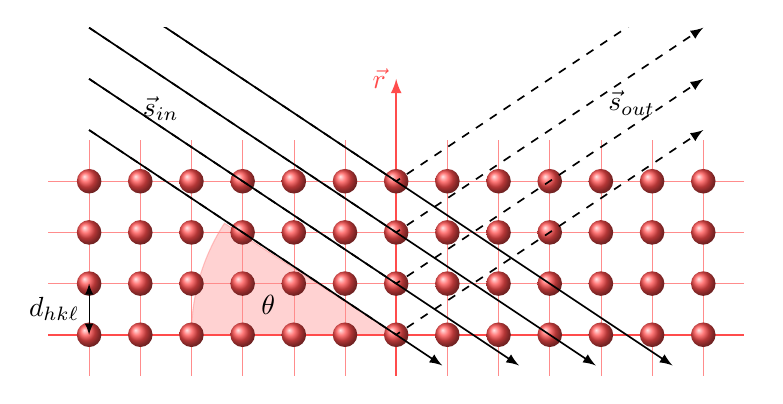
\begin{tikzpicture}[scale=1.3]
    \clip (-0.6,0.1) rectangle (6.5,3.5);

    % angle
    \filldraw[fill=red!35,draw=red!45,opacity=0.5]
    (3,0.5) -- (1,0.5) arc (180:147:2) -- cycle;
    \draw (1.75,0.6) node[above] {$\theta$};

    % grid
    \draw[style=help lines,color=red!45][step=0.5cm] (-0.4,0.1) grid (6.4,2.4);
    \draw[color=red!70, thick] (-0.4,0.5) -- (6.4,0.5);
    \draw[->, >=latex, color=red!70, thick] (3,0.1) -- (3,3) node[left] {$\vec r$};

    % atoms
    \foreach \x in {0,0.5,...,6}
    \foreach \y in {0.5,1,...,2}
    \shade[ball color=red!70] (\x,\y) circle (.12cm);

    % beams
    \foreach \y in {4,3.5,...,2.5}
    \draw[->, >=latex, semithick, dashed] (0,\y) -> +(3,-2) -> +(6,0);

    \draw[->, >=latex, semithick] (0,2.5) -> +(3.45,-2.3);
    \draw[->, >=latex, semithick] (0,3) -> +(4.2,-2.8);
    \draw[->, >=latex, semithick] (0,3.5) -> +(4.95,-3.3);
    \draw[->, >=latex, semithick] (0,4) -> +(5.7,-3.8);

    \draw (0.7,2.5) node[above] {$\vec s_{\text{in}}$};
    \draw (5.3,2.55) node[above] {$\vec s_{\text{out}}$};

    % d_h
    \draw[<->, >=latex] (0,0.5) -- (0,1) node[left,midway] {$d_{hk\ell}$};


  \end{tikzpicture}
\end{figure}

\end{frame}


\begin{frame}
  \frametitle{Diffraction Pole Figures}

  \begin{columns}
    \begin{column}{0.67\textwidth}
      \begin{itemize}
      \item<+-> For a fixed wavelength $\lambda$ and angle $2 \theta$ there is
        often only a single crystal direction
        $\vec h = (hk\ell)$ such that Braggs law is
        satisfied for the corresponding $d_{hk\ell}$.
      \item<+-> The intensity measured at the detector is proportional to the
        irradiated volume of crystals that are orientated such that the
        lattice planes $(hk\ell)$ are perpendicular to
        $\vec r = \vec s_{\text{in}} - \vec s_{\text{out}}$
      \item<+-> This corresponds to all grains with orientation $\mat O$ such that
        \begin{equation*}
          \mat O \vec h = \vec r,
        \end{equation*}
        i.e. all orientations that appear in the $\vec h = (hk\ell)$-pole figure at
        position $\vec r= \vec s_{\text{in}} - \vec s_{\text{out}}$.
      \end{itemize}
    \end{column}
    \begin{column}{0.3\textwidth}
      \vspace{-0.5cm}
      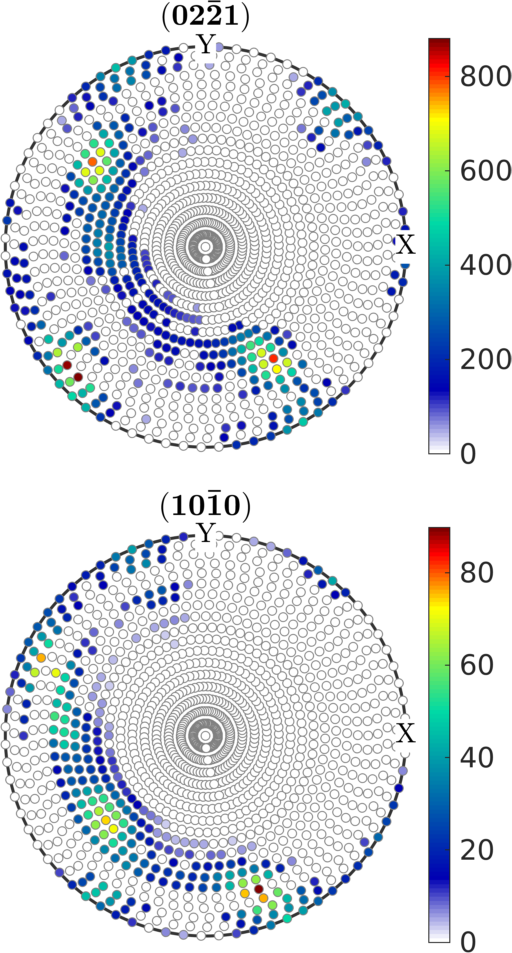
\includegraphics[width=\textwidth]{pic/pfRaw}
    \end{column}
  \end{columns}

\end{frame}


\begin{frame}
  \frametitle{The Radon Transform}

  \begin{columns}
    \begin{column}{0.6\textwidth}
      \begin{itemize}
      \item detector position $\vec r = \vec s_{\text{in}} - \vec
        s_{\text{out}}$
      \item active lattice plane $\vec h = (hk\ell)$
      \item For $N$ grains with orientations $\mat O_{n}$ and volumes $v_{n}$,
        $n=1,\ldots,N$ the intensity is proportional to
        \begin{equation*}
          I(\vec h, \vec r)
          \sim \sum_{n \colon \mat O_{n} \vec h = \vec r} v_{n}
        \end{equation*}
      \item For orientations distributed according to the ODF
        $f$ the intensity is proportional to
        \begin{equation*}
          I(\vec h, \vec r) \sim
          \mathcal R f(\vec h, \vec r)
          = \int_{\mat O \vec h = \vec r} f(\mat O) \mathrm d \mat O
        \end{equation*}
      \item<2> The integral is called Radon transform of the ODF $f$
        and $\mathcal R f(\vec h, \cdot)$ the $(hk\ell)$ pole density function.
      \end{itemize}
    \end{column}
      \begin{column}{0.36\textwidth}

    \begin{overlayarea}{\textwidth}{0.85\textheight}
    \vspace{-1cm}%
    \centering%
    \only<1>{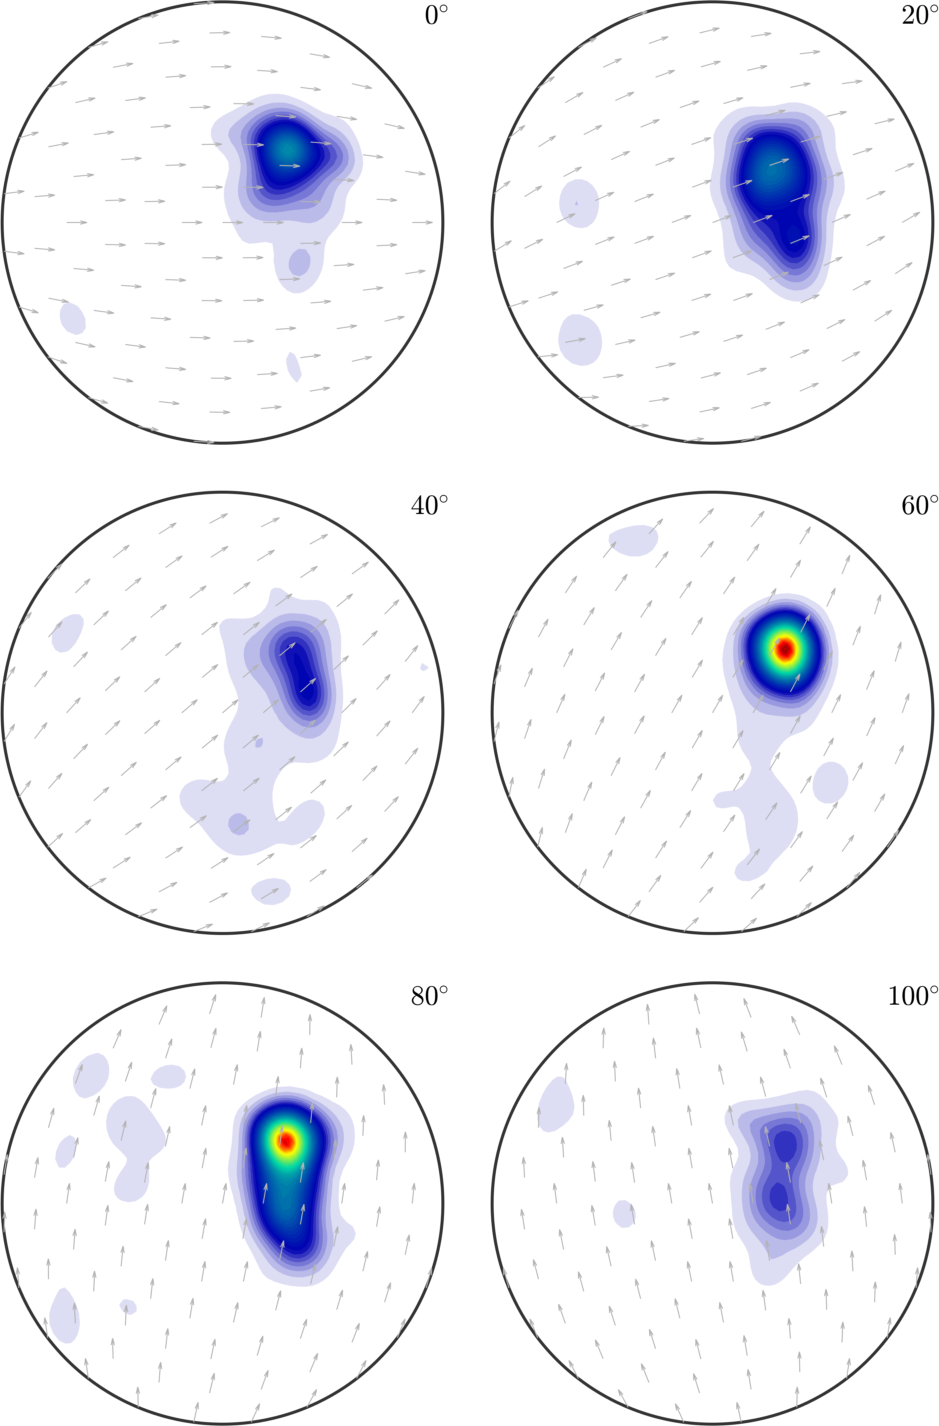
\includegraphics[width=\textwidth]{pic/odfRec}}%
    \only<2>{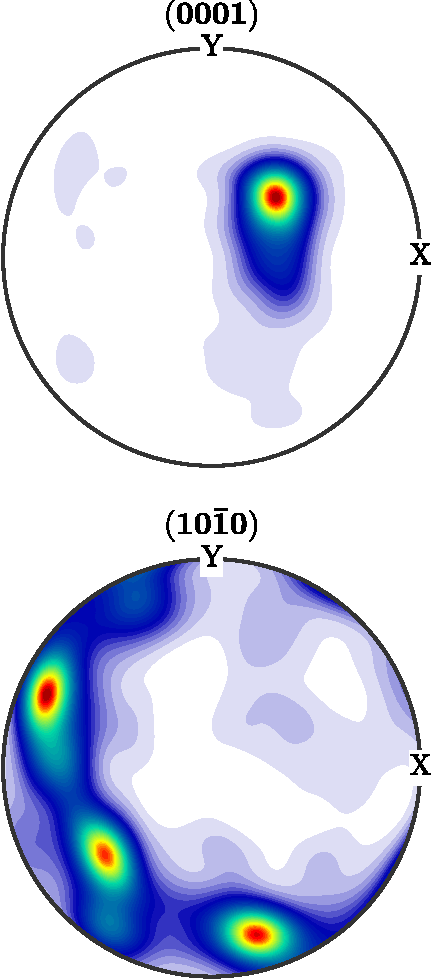
\includegraphics[width=0.68\textwidth]{pic/pfRec.pdf}}
  \end{overlayarea}
\end{column}
  \end{columns}
\end{frame}

\begin{frame}[fragile]
  \frametitle{The Pole Density Function in MTEX}


  \begin{columns}
    \begin{column}{0.6\textwidth}
      \begin{overlayarea}{\textwidth}{0.85\textheight}
        \begin{lstlisting}[style=input]
cs = crystalSymmetry.load('quartz')
plot(odf,'sigma')
\end{lstlisting}

\pause

\begin{lstlisting}[style=input]
h = Miller({0,0,0,1},{1,0,-1,0},cs)
plotPDF(odf,h)
\end{lstlisting}

\pause

        \begin{lstlisting}[style=input]
pdf = calcPDF(odf,h(2))
[m,pos] = max(pdf,'numLocal',3)
\end{lstlisting}

\pause

        \begin{lstlisting}[style=input]
pdf = calcPDF(odf,h(1))
[m,pos] = max(pdf)
f = fibre(h(1),pos)
plot(odf,f)
\end{lstlisting}




      \end{overlayarea}
  \end{column}
  \begin{column}{0.36\textwidth}

    \begin{overlayarea}{\textwidth}{0.85\textheight}
    \vspace{-1cm}%
    \centering%
    \only<1>{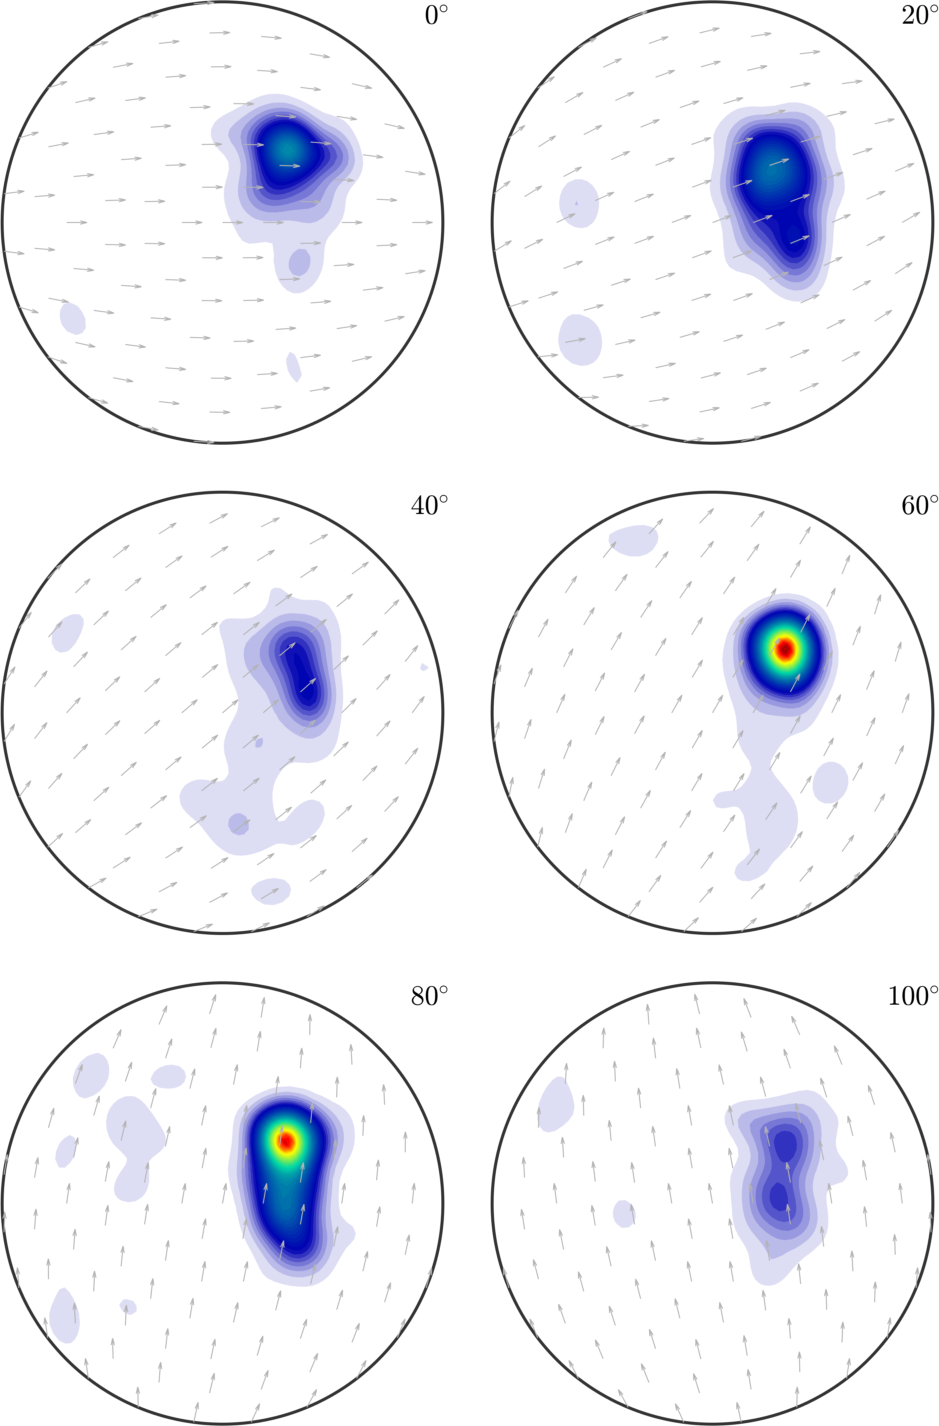
\includegraphics[width=\textwidth]{pic/odfRec}}%
    \only<2>{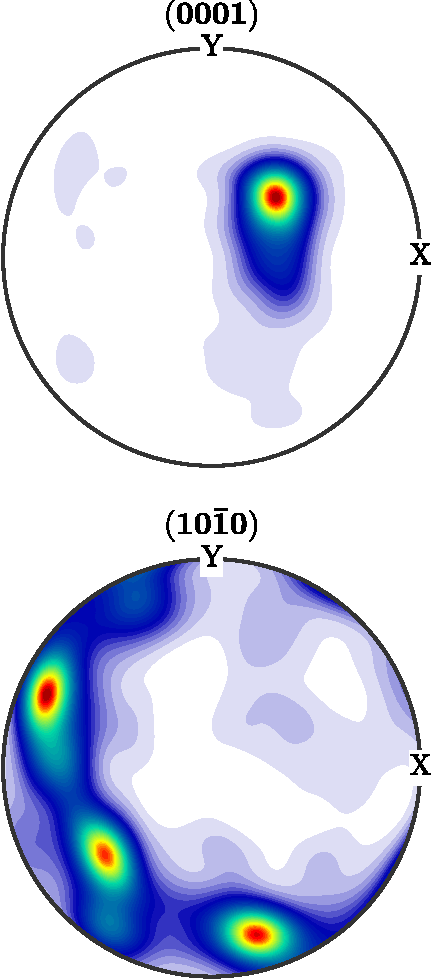
\includegraphics[width=0.68\textwidth]{pic/pfRec.pdf}}
    \only<3>{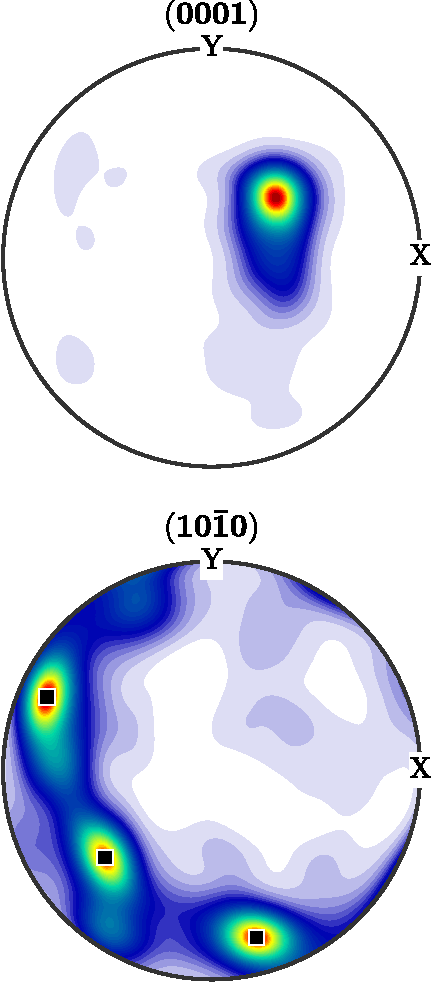
\includegraphics[width=0.68\textwidth]{pic/pfRecMarked.pdf}}
    \only<4>{\vspace{3cm}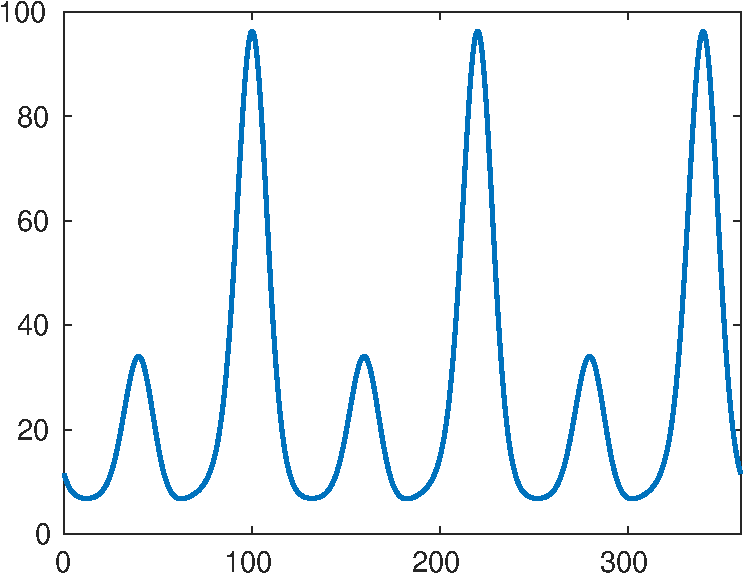
\includegraphics[width=\textwidth]{pic/fibre.pdf}}
  \end{overlayarea}
\end{column}
  \end{columns}


\end{frame}



\begin{frame}[fragile]
  \frametitle{Importing Pole Figure Data}

  \begin{columns}%
    \begin{column}{0.65\textwidth}%
      \begin{overlayarea}{\textwidth}{0.85\textheight}%
        \vspace{-0.5cm}%
        \begin{lstlisting}[style=input]
CS = crystalSymmetry.load('quartz')

% lattice planes
h = {Miller(1,0,-1,0,CS),...
  Miller({0,1,-1,1},{1,0,-1,1},CS)}

% structure coefficients
c = {1,[0.52 ,1.23]};

% import data
pf = PoleFigure.load(fnames,h,...
                'superposition',c)
              \end{lstlisting}
              \vspace{-0.4cm}%
              \begin{lstlisting}[style=output]
pf = /+PoleFigure+/
  crystal symmetry : -3m1, X||a*, Y||b, Z||c*
  specimen symmetry: 1

  h = (10-10), r = 72 x 19 points
  h = (01-11)(10-11), r = 72 x 19 points
              \end{lstlisting}
      \end{overlayarea}
    \end{column}

  \begin{column}{0.3\textwidth}

    \begin{overlayarea}{\textwidth}{0.85\textheight}
      \vspace{-1cm}%
      \centering%
      \only<1>{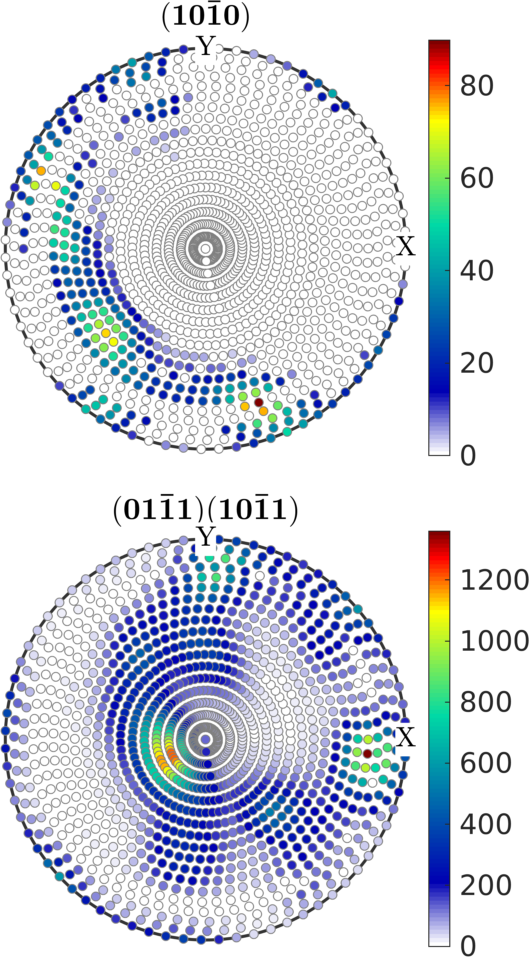
\includegraphics[width=\textwidth]{pic/pfRaw2}}%
    \end{overlayarea}
  \end{column}
  \end{columns}
  \end{frame}

\begin{frame}[fragile]
  \frametitle{Modifying Pole Figure Data}

    \begin{columns}%
    \begin{column}{0.65\textwidth}%
      \begin{overlayarea}{\textwidth}{0.85\textheight}%
        rotate \vspace{-0.2cm}
        \begin{lstlisting}[style=input]
pfRot = rot * pf
\end{lstlisting}

\pause

scale \vspace{-0.2cm}
\begin{lstlisting}[style=input]
pf = [1 0.1] * pf
\end{lstlisting}

\pause

normalize \vspace{-0.2cm}
\begin{lstlisting}[style=input]
pf = pf.normalize
\end{lstlisting}

\pause

properties \vspace{-0.2cm}
\begin{lstlisting}[style=input]
pf.intensities, pf.r, pf.h, pf.CS
\end{lstlisting}

\pause

modify \vspace{-0.2cm}
\begin{lstlisting}[style=input]
pf(pf.intensities<0) = 0
pf(pf.isOutlier) = []
\end{lstlisting}

\pause

first pole figure \vspace{-0.2cm}
\begin{lstlisting}[style=input]
pf{1}
\end{lstlisting}

      \end{overlayarea}
    \end{column}
      \begin{column}{0.3\textwidth}

    \begin{overlayarea}{\textwidth}{0.85\textheight}
      \vspace{-1cm}%
      \centering%
      \only<1>{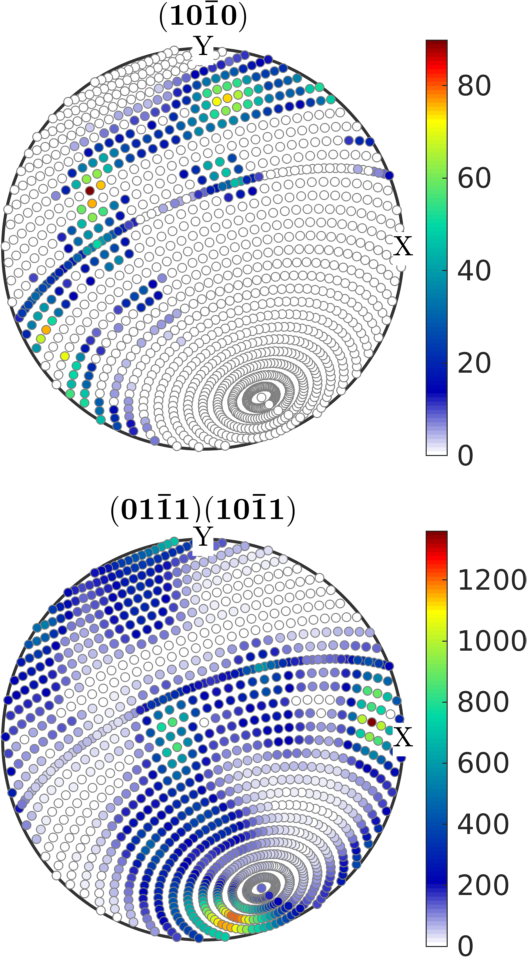
\includegraphics[width=\textwidth]{pic/pfRot}}%
      \only<2>{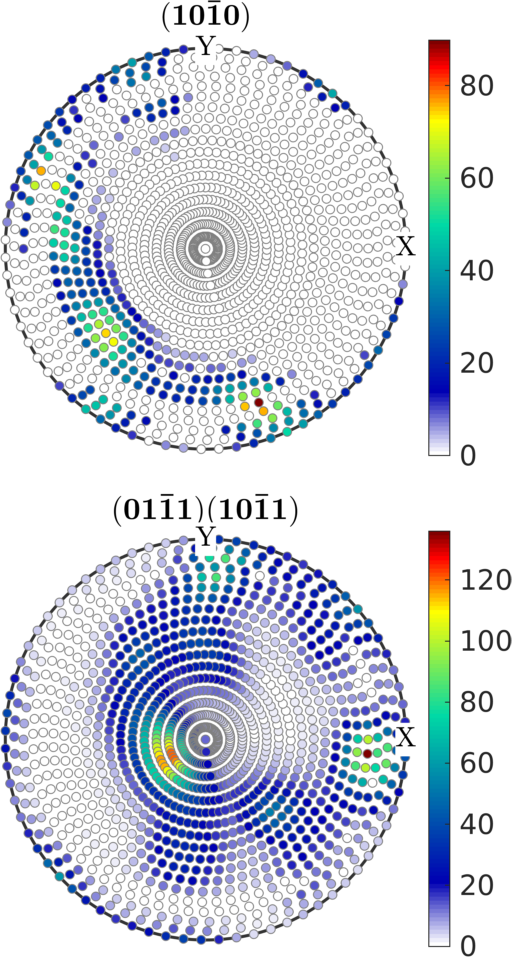
\includegraphics[width=0.98\textwidth]{pic/pfScaled}}%
      \only<3->{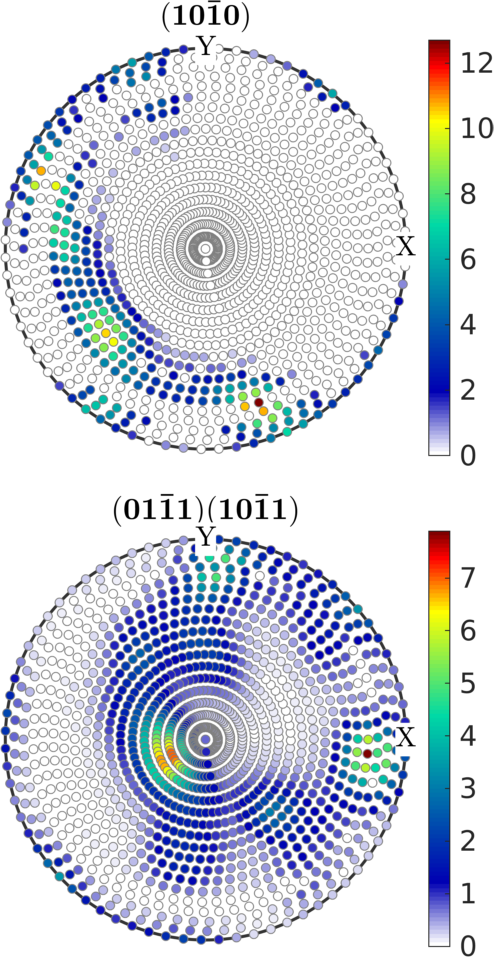
\includegraphics[width=0.95\textwidth]{pic/pfNorm}}%
    \end{overlayarea}
  \end{column}
\end{columns}

\end{frame}


\begin{frame}[fragile]

  \frametitle{Background and Defocusing Correction}

    \begin{columns}%
    \begin{column}{0.65\textwidth}%
      \begin{overlayarea}{\textwidth}{0.85\textheight}%
        the data \vspace{-0.2cm}
\begin{lstlisting}[style=output]
pf = /+PoleFigure+/
  crystal symmetry : m-3m
  specimen symmetry: 1

  h = (104), r = 679 x 1 points
  h = (104), r = 16 x 1 points
  h = (110), r = 679 x 1 points
  h = (110), r = 16 x 1 points
\end{lstlisting}

\pause

background correction \vspace{-0.2cm}
\begin{lstlisting}[style=input]
pf = correct(pf{[1,3]},'bg',pf{[2,4]})
\end{lstlisting}

\pause

defocusing correction \vspace{-0.2cm}
\begin{lstlisting}[style=input]
pf = correct(pf,'bg',pf_bg,...
  'def',def,'defbg',pf_defbg)
\end{lstlisting}

\pause

by function \vspace{-0.2cm}
\begin{lstlisting}[style=input]
pf = pf .* myCorrectionFun(pf.r.theta)
\end{lstlisting}


      \end{overlayarea}
    \end{column}
      \begin{column}{0.3\textwidth}

    \begin{overlayarea}{\textwidth}{0.85\textheight}
      \vspace{-1cm}%
      \centering%
      \only<1>{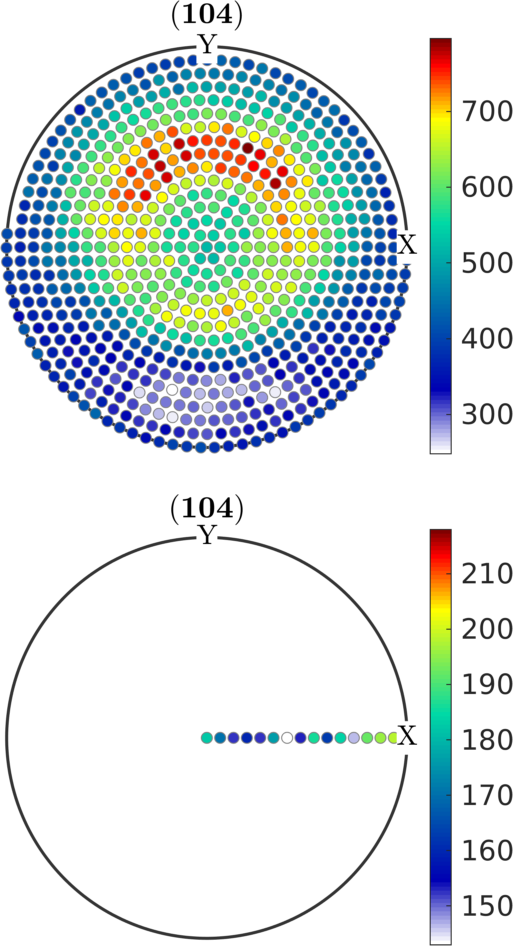
\includegraphics[width=\textwidth]{pic/pfGeest}}%
      \only<2->{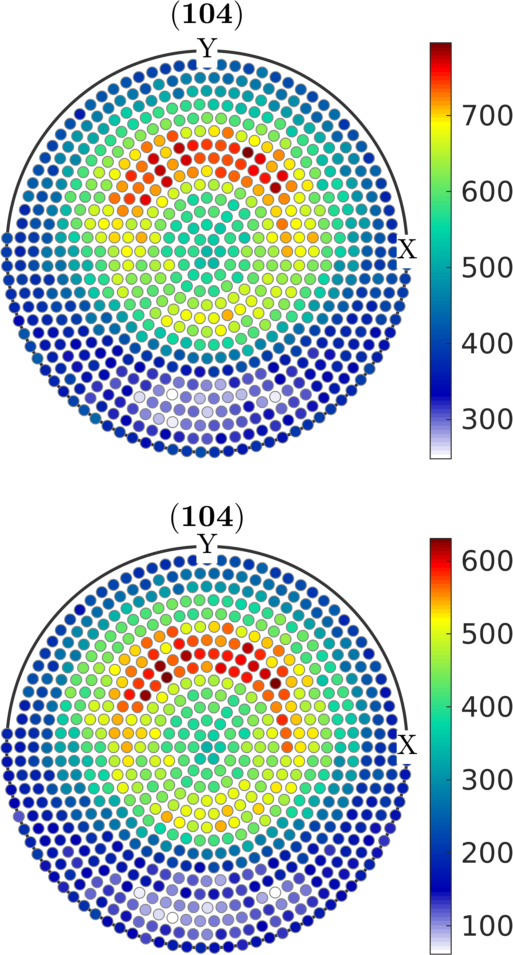
\includegraphics[width=0.98\textwidth]{pic/pfGeestCor}}%
    \end{overlayarea}
  \end{column}
\end{columns}

\end{frame}


\begin{frame}[fragile]
  \frametitle{ODF Reconstruction from Pole Figure Data}



    \begin{columns}%
    \begin{column}{0.65\textwidth}%
      \begin{overlayarea}{\textwidth}{0.85\textheight}%
        the data \vspace{-0.2cm}
        \begin{lstlisting}[style=output]
pf = /+PoleFigure+/
  crystal symmetry : Quartz (321, X||a*, Y||b, Z||c*)
  specimen symmetry: 1

  h = (02-21), r = 72 x 19 points
  h = (10-10), r = 72 x 19 points
  h = (10-11)(01-11), r = 72 x 19 points
  h = (10-12), r = 72 x 19 points
  h = (11-20), r = 72 x 19 points
  h = (11-21), r = 72 x 19 points
\end{lstlisting}

\begin{onlyenv}<2->
odf reconstruction \vspace{-0.2cm}
\begin{lstlisting}[style=input]
odf = calcODF(pf)
\end{lstlisting}
\end{onlyenv}
\begin{onlyenv}<2>
\vspace{-0.4cm}
\begin{lstlisting}[style=output]
odf = /+ODF+/
  crystal symmetry : Quartz (321, X||a*, Y||b, Z||c*)

  Radially symmetric portion:
    kernel: de la Vallee Poussin, halfwidth 5
    center: 19836 orientations, resolution: 5
    weight: 1
\end{lstlisting}
  \end{onlyenv}

\begin{onlyenv}<3->
\begin{lstlisting}[style=input]
plotPDF(odf,pf.h(1:6))
\end{lstlisting}
\end{onlyenv}
\end{overlayarea}
    \end{column}
      \begin{column}{0.33\textwidth}

    \begin{overlayarea}{\textwidth}{0.85\textheight}
      \vspace{-1cm}%
      \centering%
      \only<1>{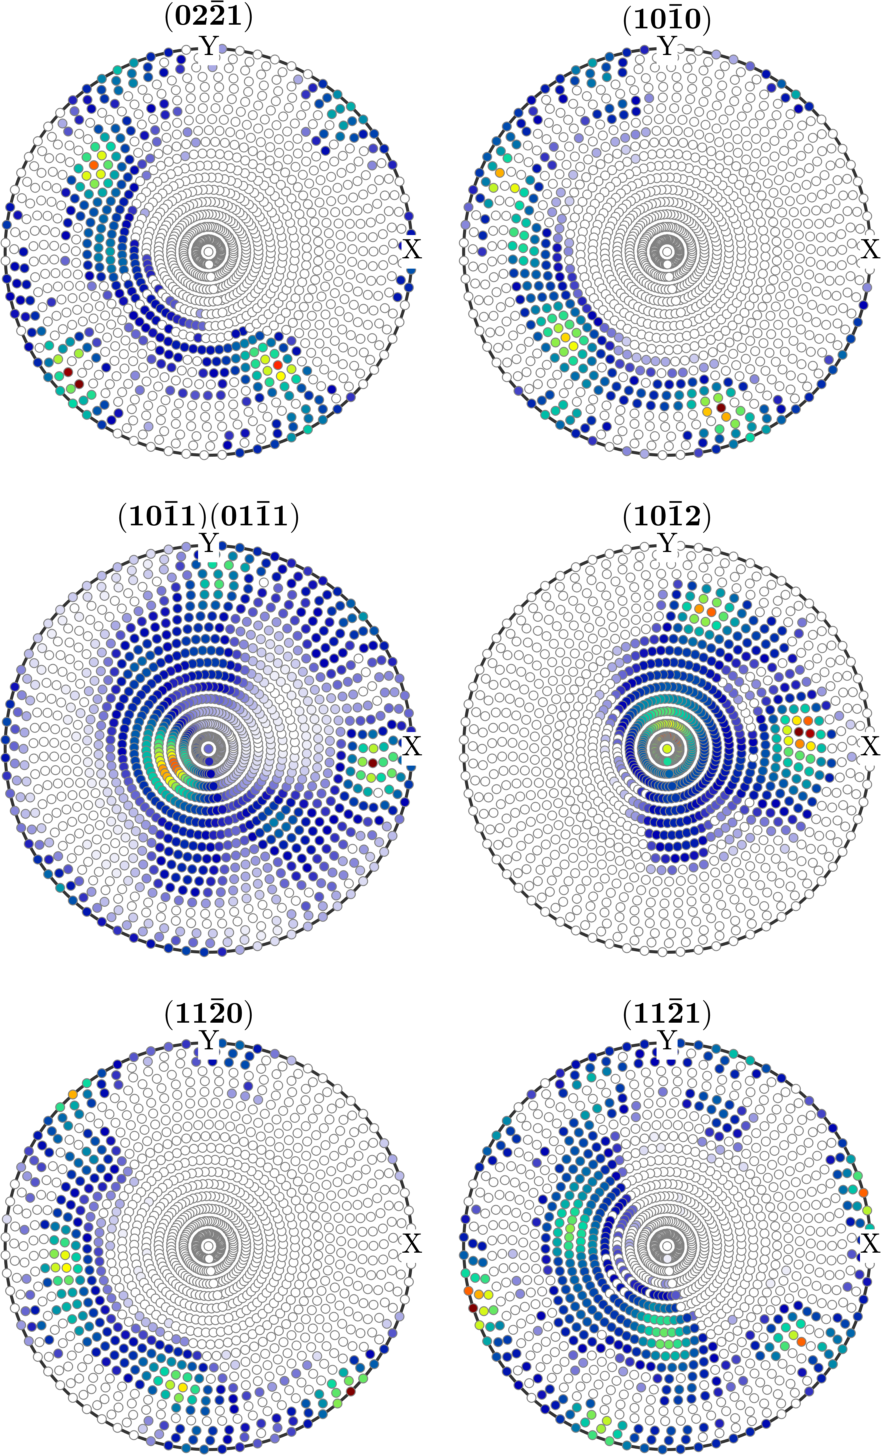
\includegraphics[width=\textwidth]{pic/pfRaw6}}%
      \begin{onlyenv}<2>
        \vspace{0.9cm}
        \begin{lstlisting}[style=output]
0 | 0.89 0.91 0.77 1.12 0.90
1 | 0.87 0.87 0.66 1.02 0.90
2 | 0.84 0.82 0.54 0.93 0.88
3 | 0.76 0.73 0.43 0.83 0.83
4 | 0.67 0.66 0.41 0.76 0.79
5 | 0.65 0.63 0.40 0.74 0.78
6 | 0.64 0.62 0.39 0.73 0.77
\end{lstlisting}

options:
\vspace{-0.2cm}
\begin{lstlisting}[style=input]
'halfwidth' 'kernel'
'iterMin' 'iterMax'
'resolution'
'zeroRange'
'noGhostCorrection'
\end{lstlisting}

        \end{onlyenv}
      \only<3>{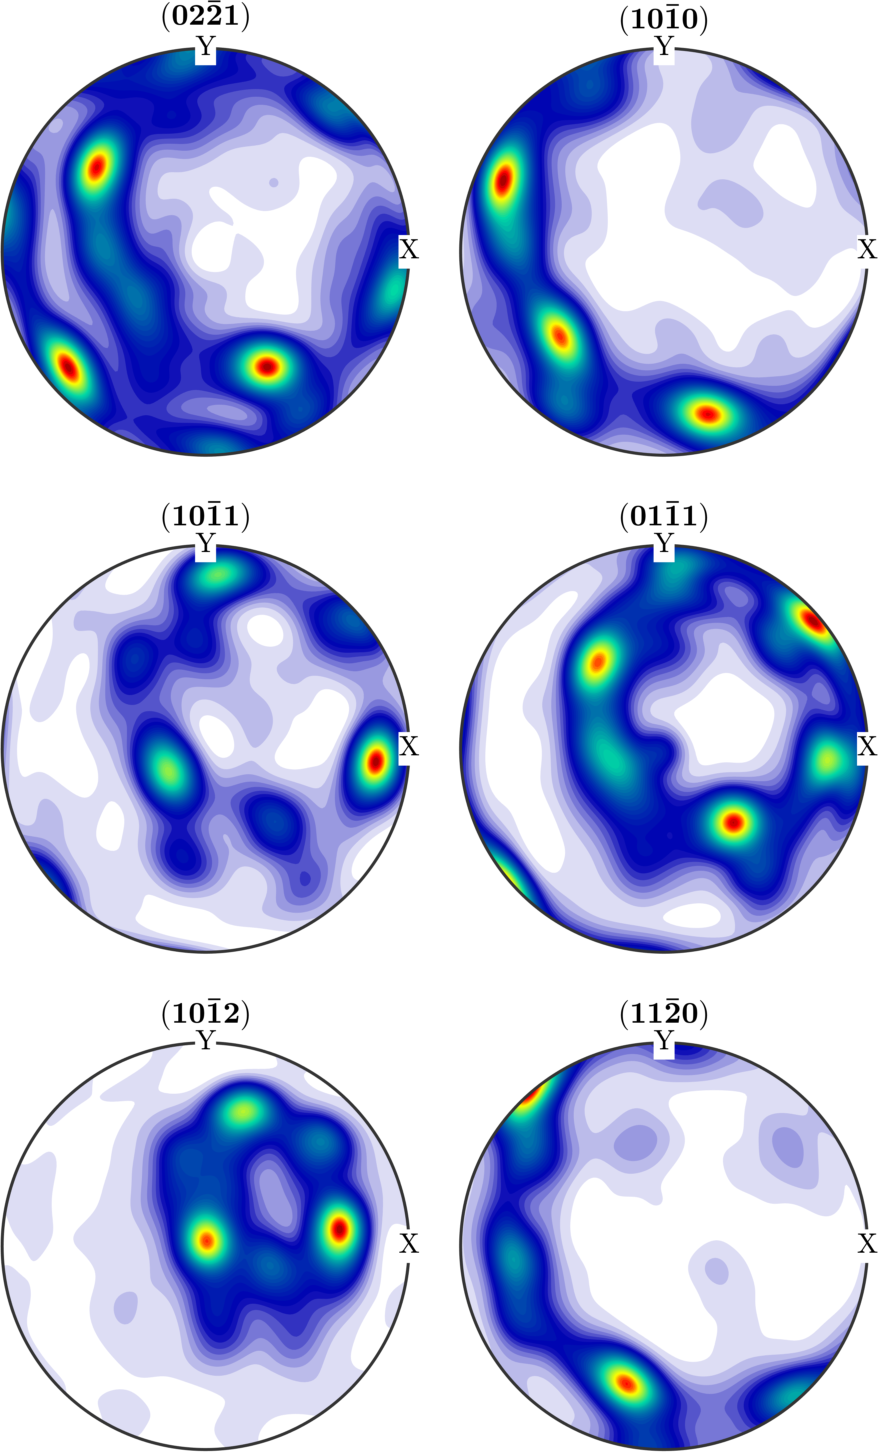
\includegraphics[width=\textwidth]{pic/pfRec6}}%
    \end{overlayarea}
  \end{column}
\end{columns}

\end{frame}


\begin{frame}[fragile]
  \frametitle{The Ambiguity of the ODF Reconstruction Problem}


  \begin{columns}
    \begin{column}{0.525\textwidth}

      The following two ODFs
\vspace{-0.2cm}
      \begin{lstlisting}[style = input]
ax   = [xvector, yvector, zvector]
ori2 = orientation.byAxisAngle(...
       ax, 90*degree,cs)
odf2 = unimodalODF(ori)
\end{lstlisting}

\pause

      \begin{lstlisting}[style = input]
ax   = vector3d(1,1,1)
ori2 = orientation.byAxisAngle(...
       ax, [0 120 240]*degree,cs)
odf2 = unimodalODF(ori)
      \end{lstlisting}

      \pause

      have \textbf{7} identical pole figures
      \vspace{-0.2cm}
      \begin{lstlisting}[style=input]
h = Miller({1,0,0},{0,1,0},...
   {0,0,1},{1,1,0},{1,0,1},...
   {0,1,1},{1,1,1},cs)
plotPDF(odf1,h)
      \end{lstlisting}



    \end{column}
    \begin{column}{0.45\textwidth}
      \only<1>{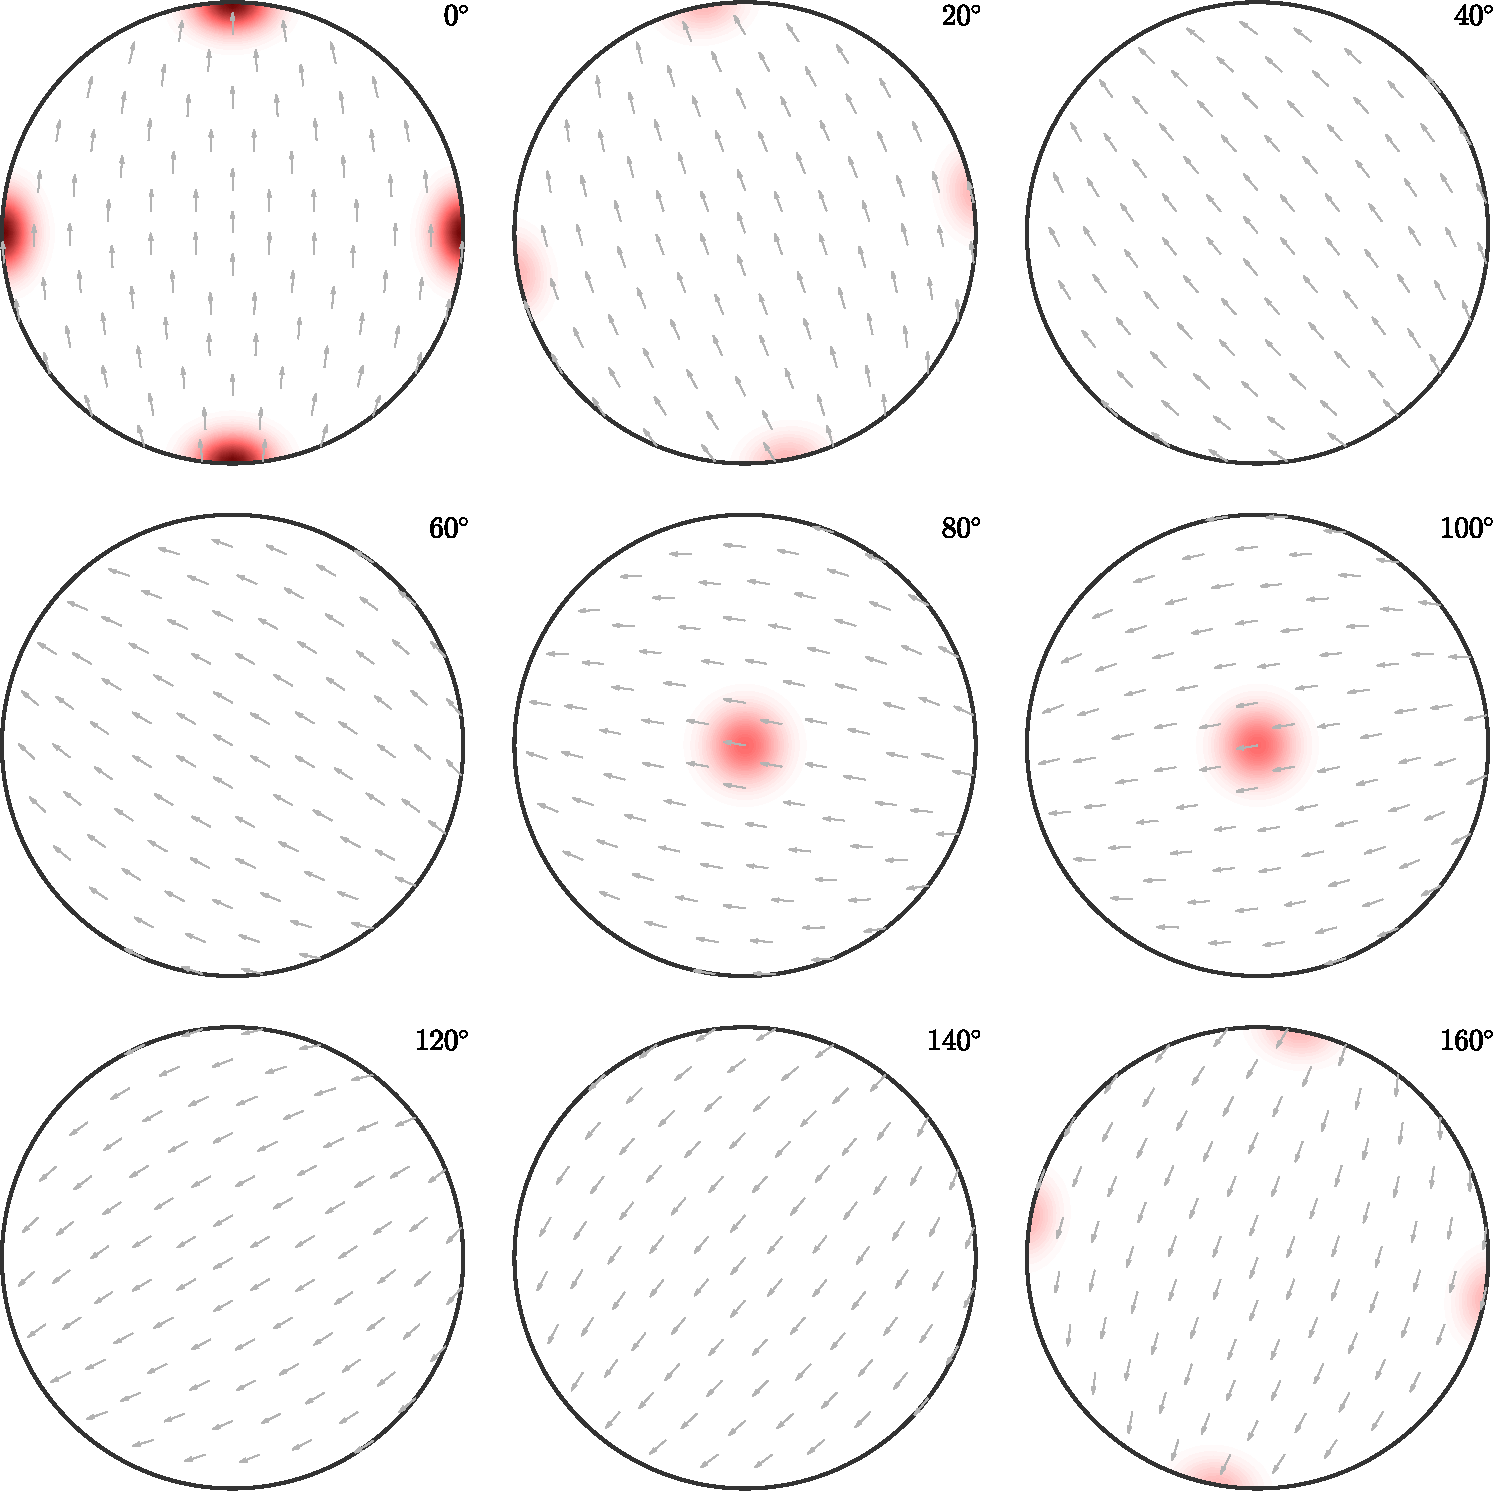
\includegraphics[width=\textwidth]{pic/ODF1}}
      \only<2>{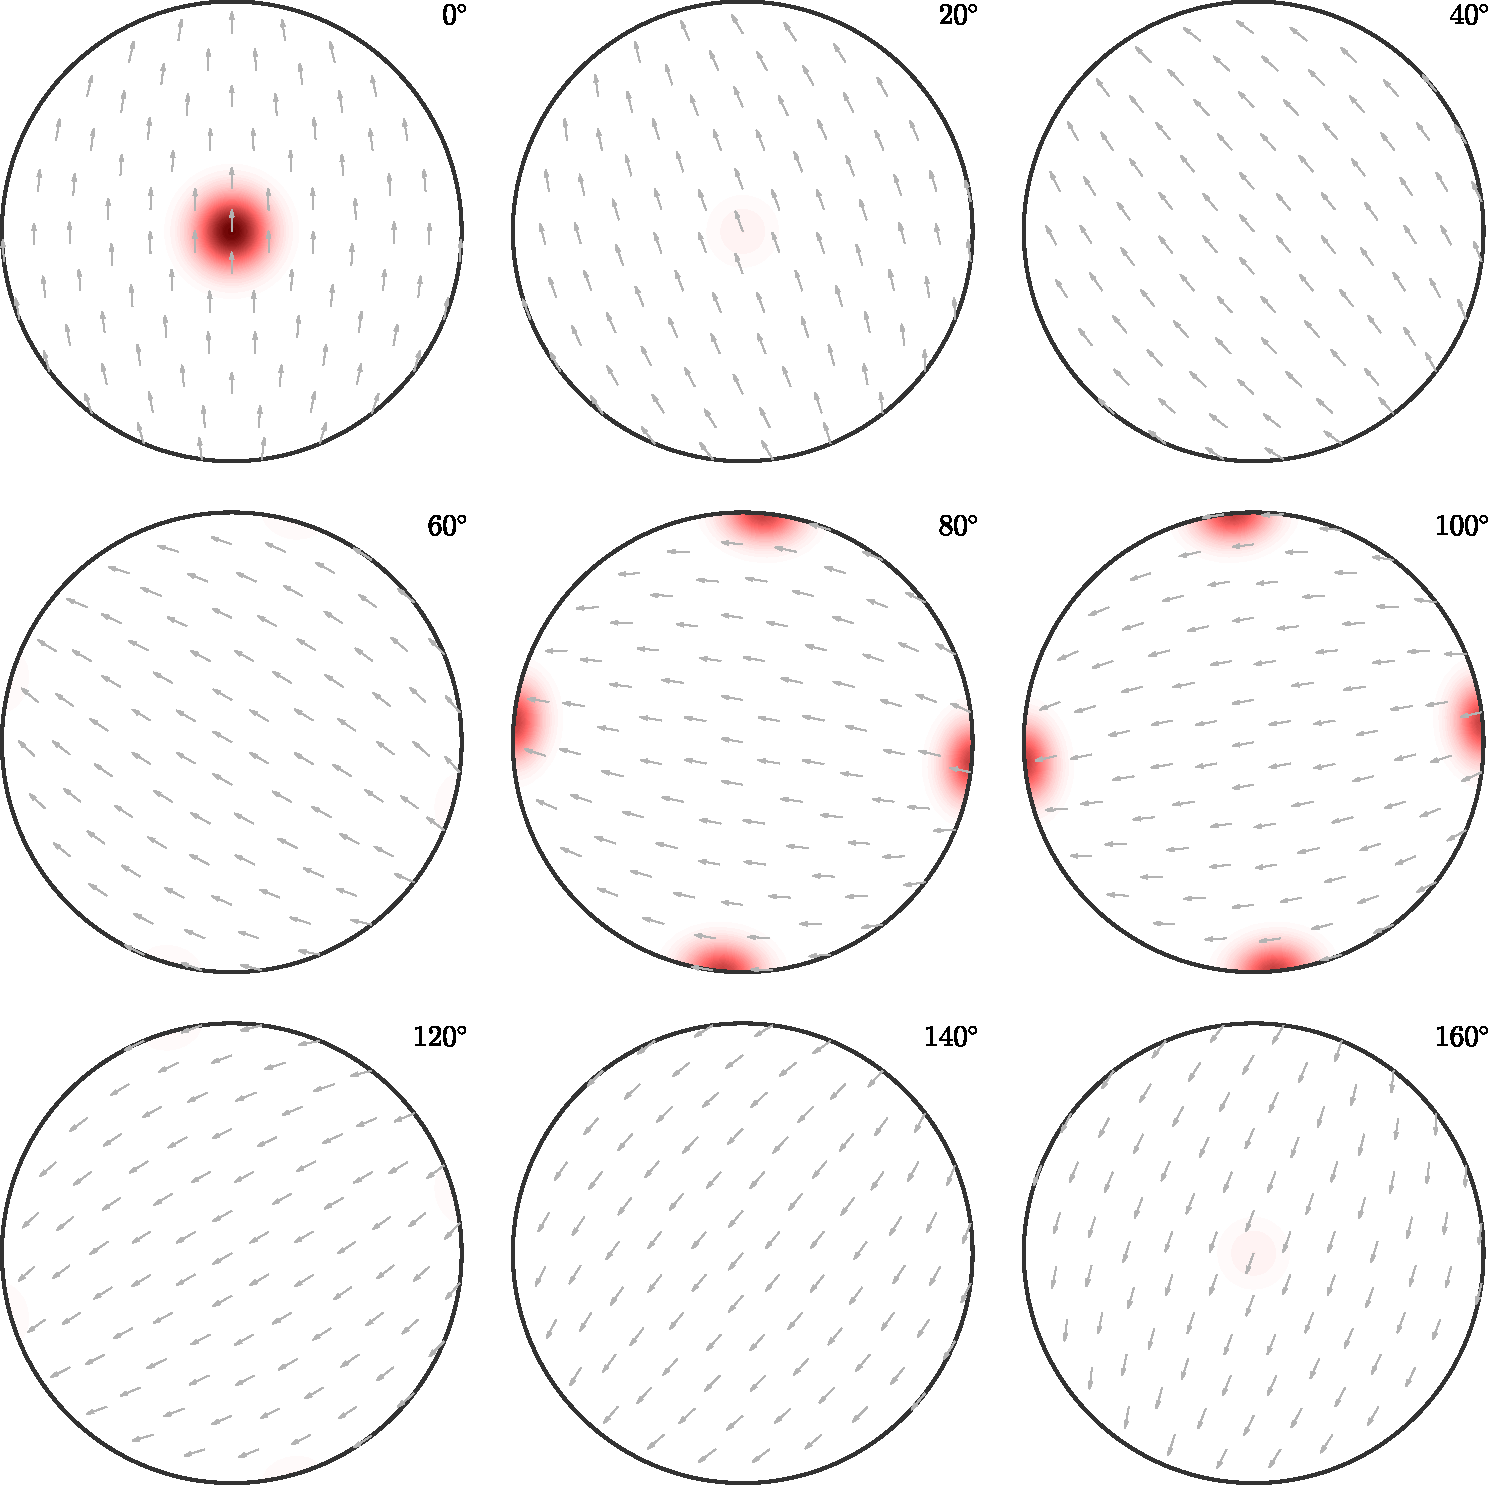
\includegraphics[width=\textwidth]{pic/ODF2}}
      \only<3>{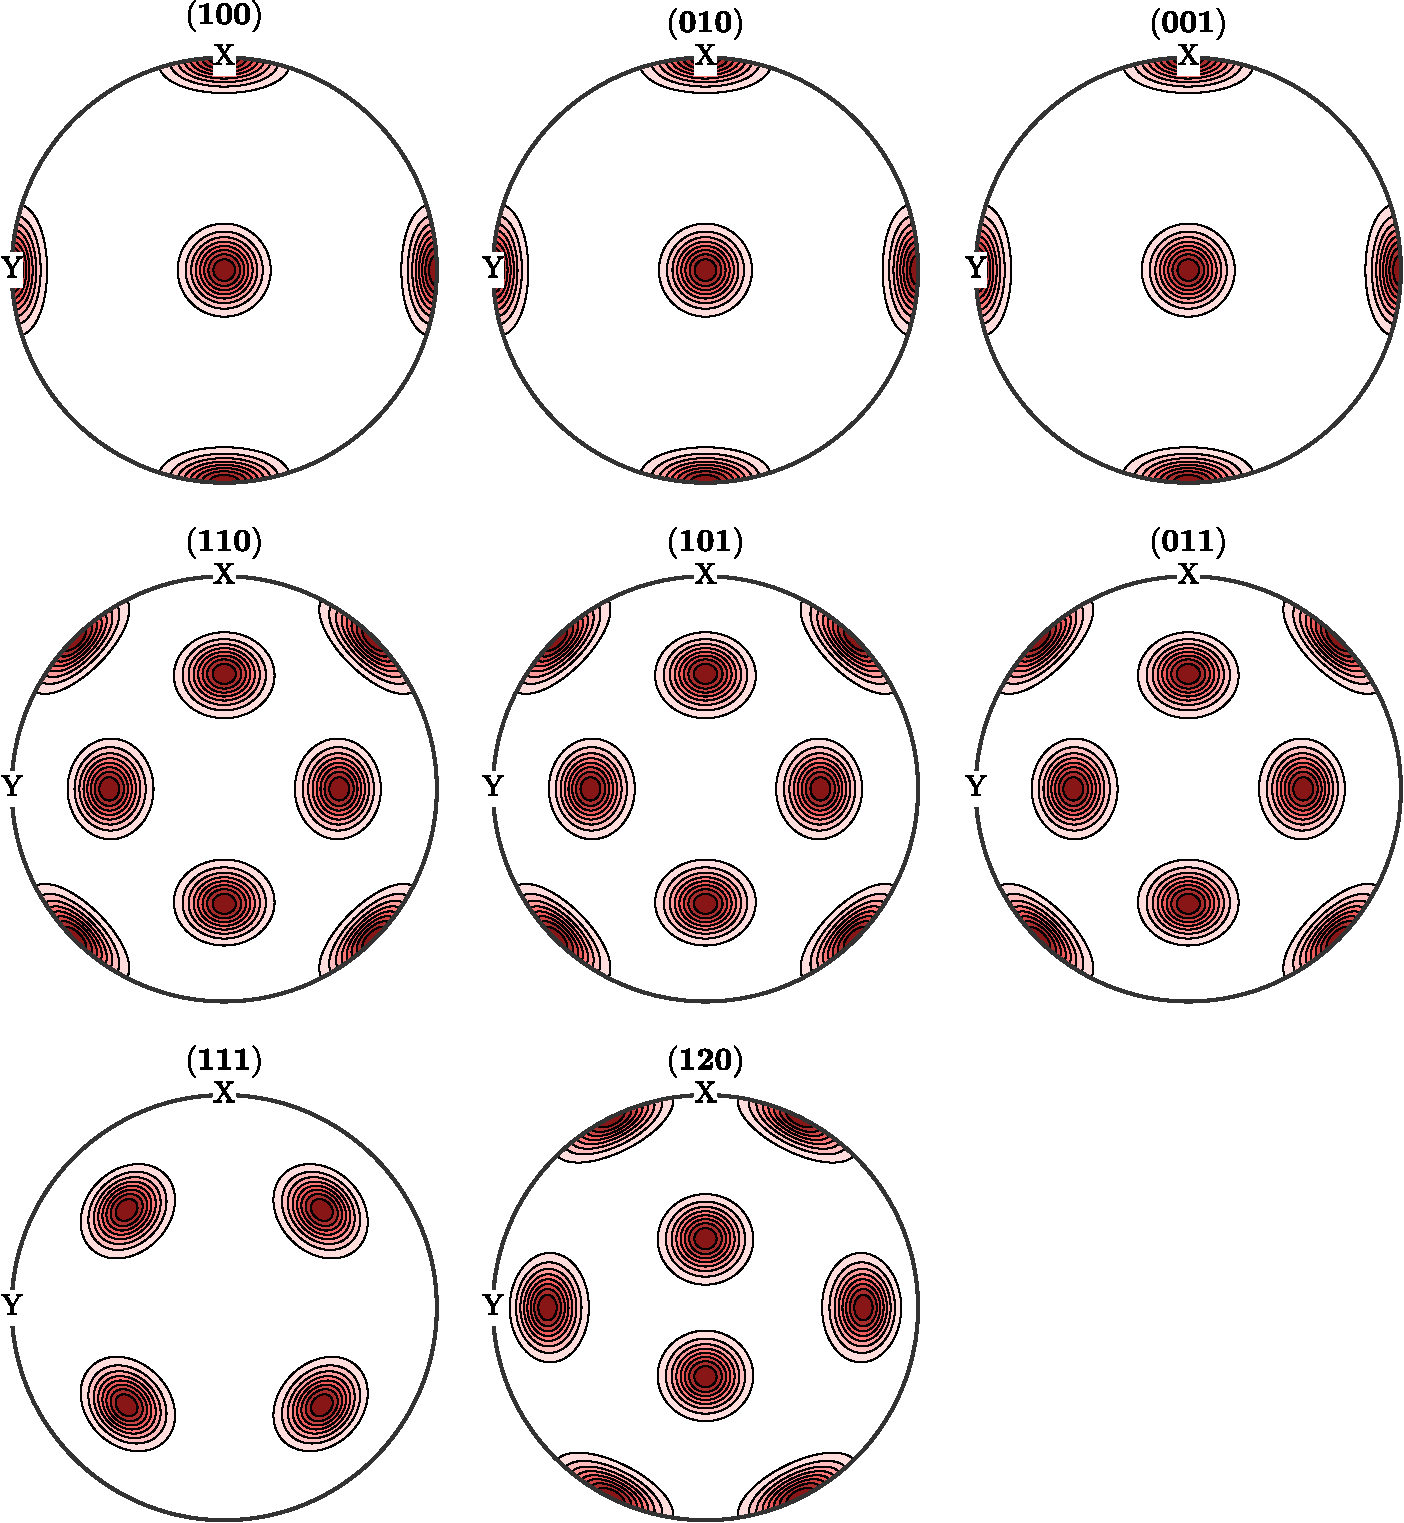
\includegraphics[width=\textwidth]{pic/pfODF1}}
      \only<4>{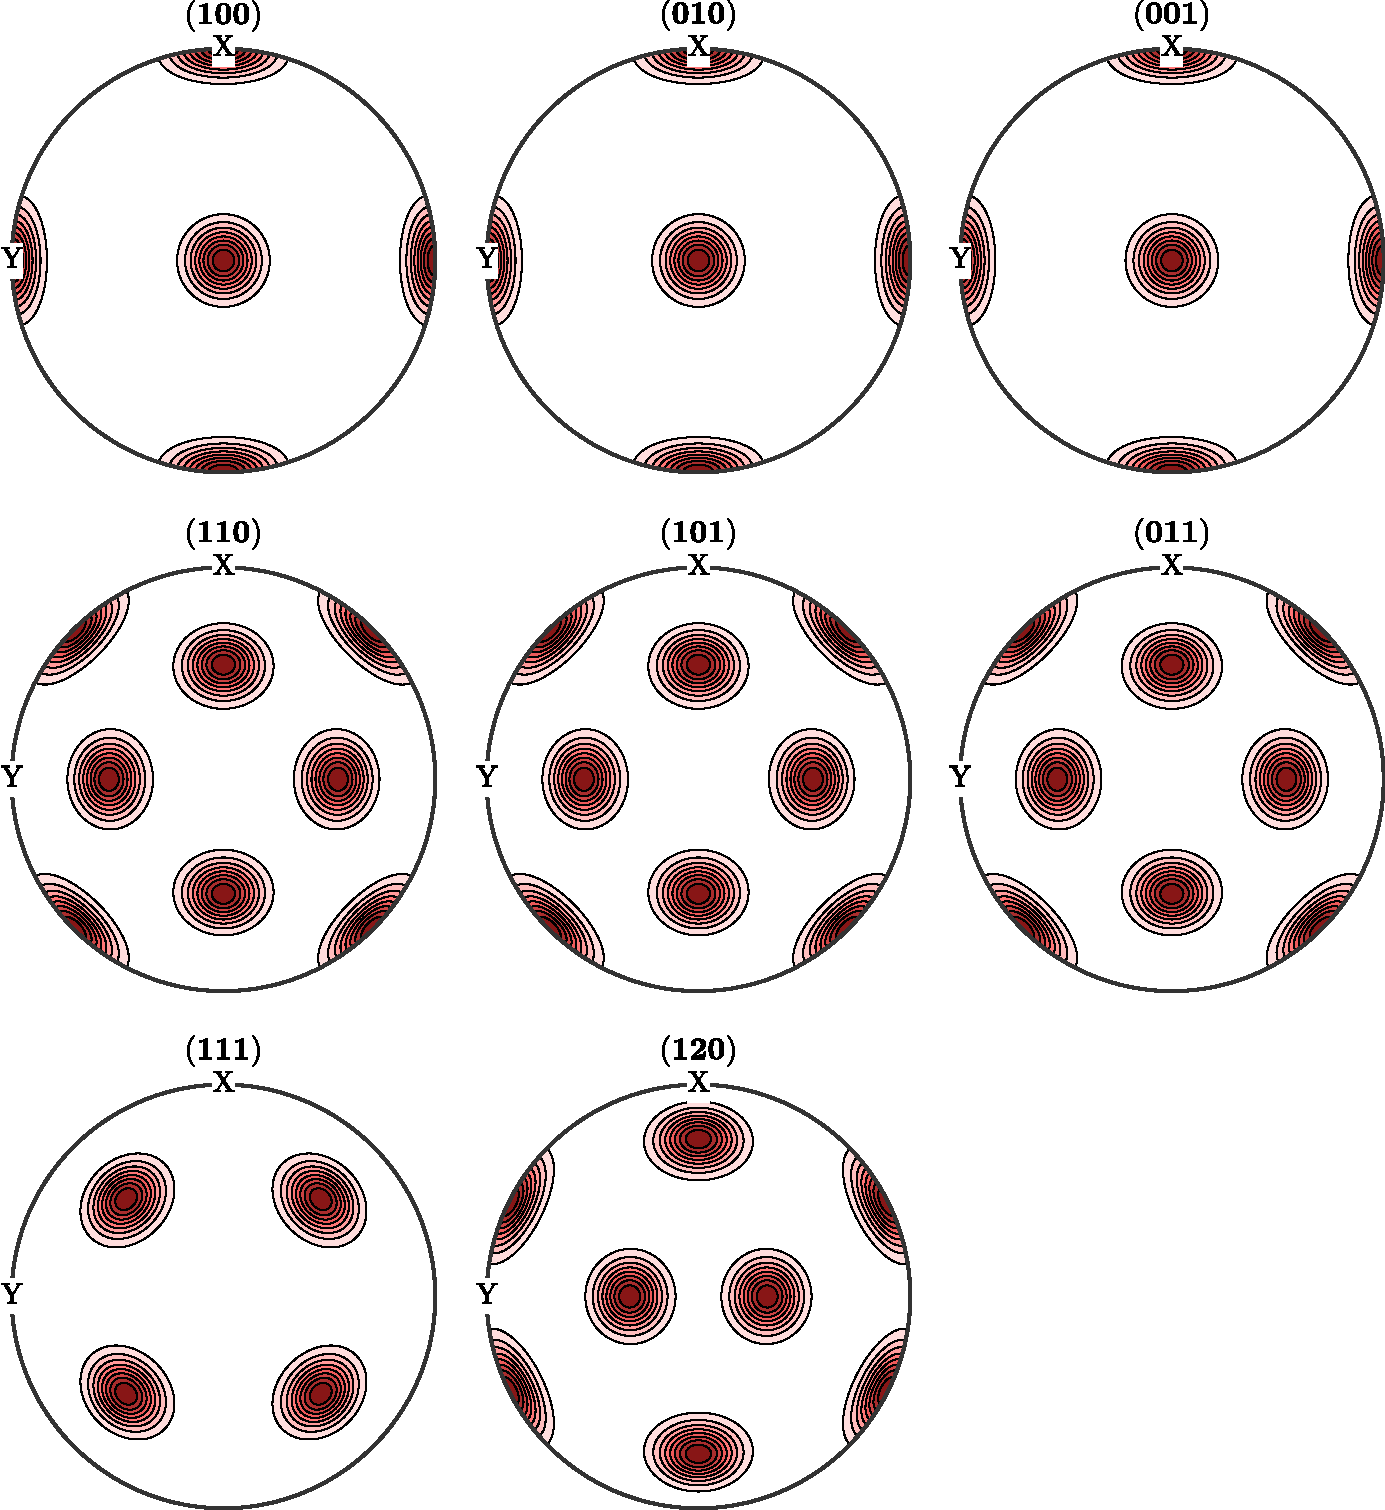
\includegraphics[width=\textwidth]{pic/pfODF2}}
      \only<5>{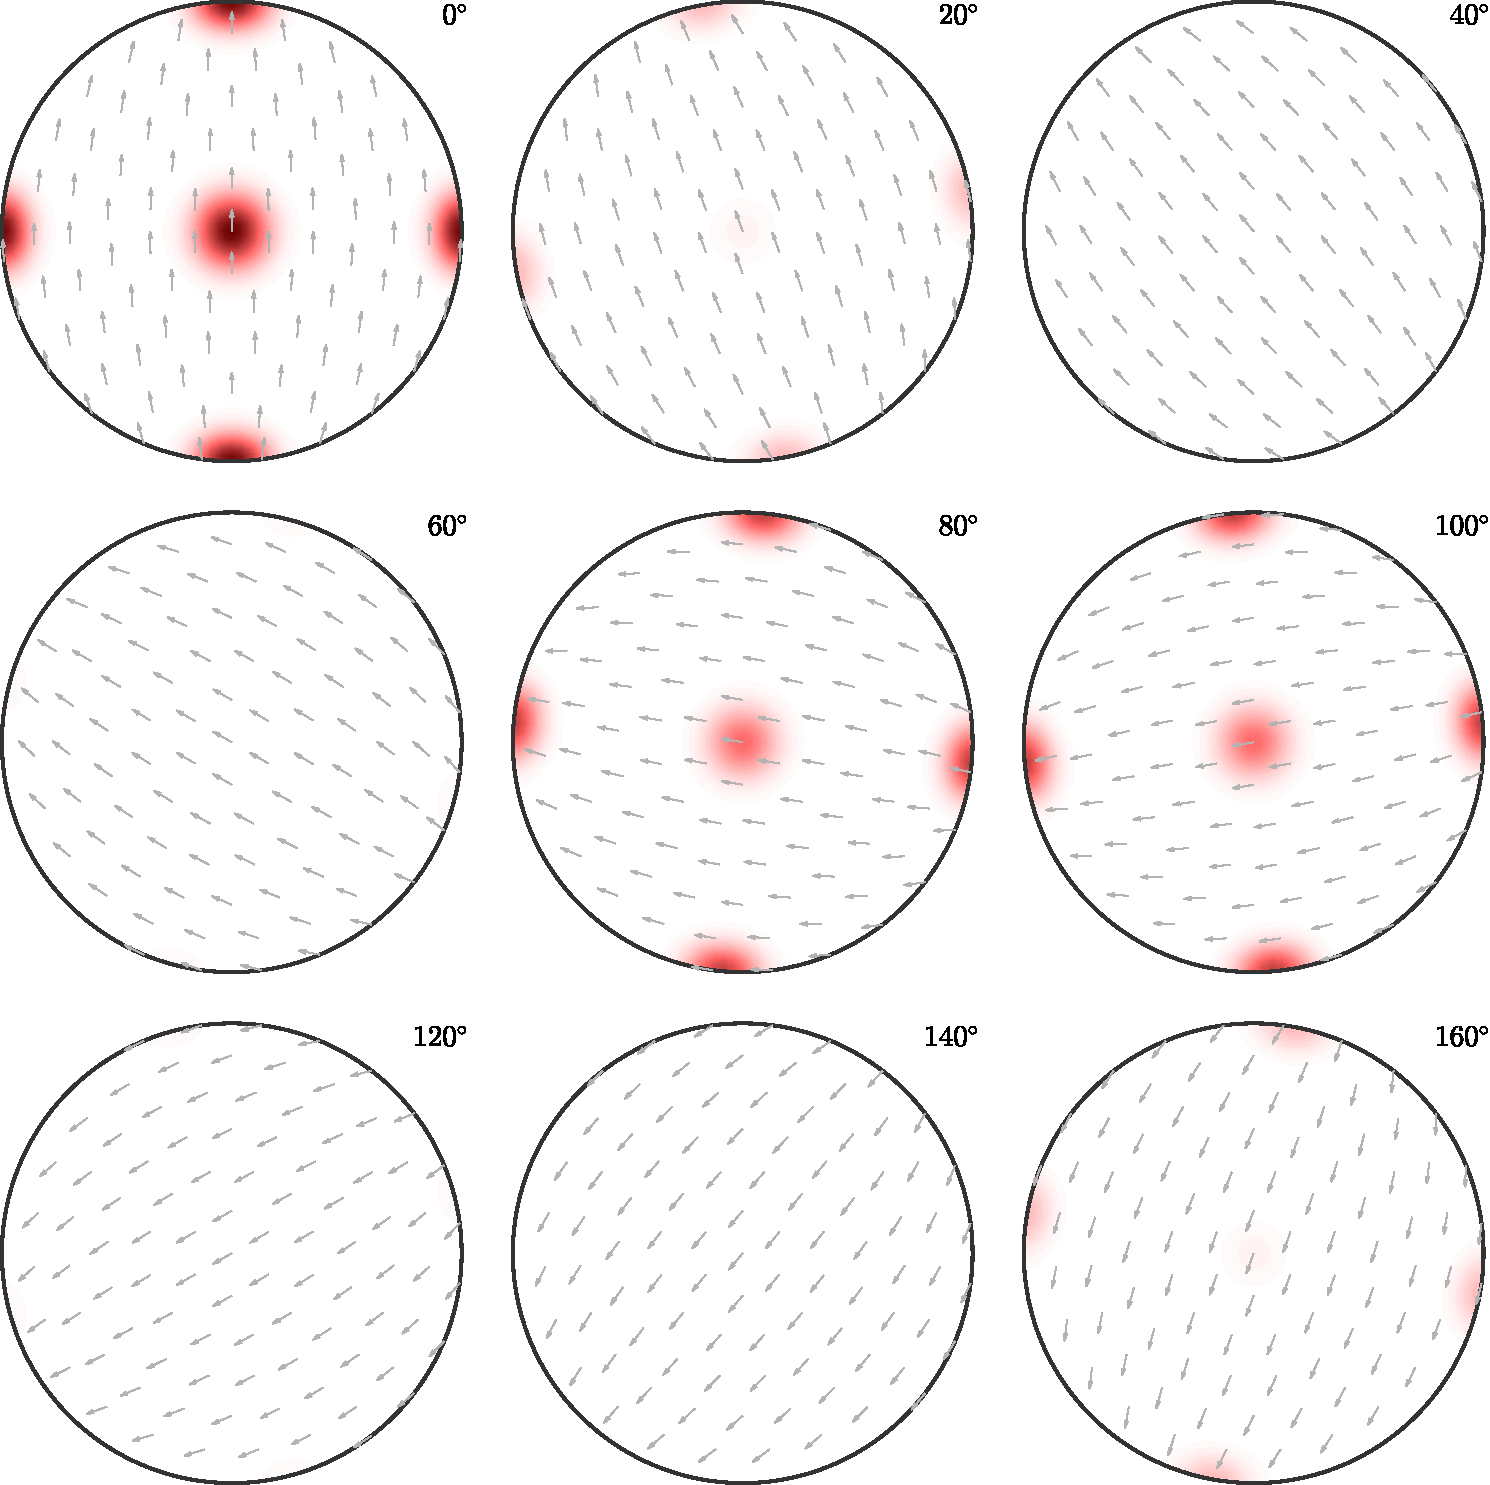
\includegraphics[width=\textwidth]{pic/pfODF3}}
    \end{column}
  \end{columns}



\end{frame}


\begin{frame}[fragile]
  \frametitle{The Even / Odd Problem}

  \begin{columns}
    \begin{column}{0.56\textwidth}

      the famous SantaFe sample odf \vspace{-0.2cm}
      \begin{lstlisting}[style=input]
plot(SantaFe,'layout',[4 3])
      \end{lstlisting}

\pause

simulate discrete pole figures \vspace{-0.2cm}
      \begin{lstlisting}[style=input]
pf = calcPoleFigure(odf,h)
\end{lstlisting}

\pause

odf reconstruction without ghost correction \vspace{-0.2cm}
      \begin{lstlisting}[style=input]
rec = calcODF(pf,'noGhostCorrection')
\end{lstlisting}

\pause

odf reconstruction with ghost correction \vspace{-0.2cm}
      \begin{lstlisting}[style=input]
rec6 = calcODF(pf)
\end{lstlisting}

\pause

odf reconstruction with 2 pole figures \vspace{-0.2cm}
      \begin{lstlisting}[style=input]
rec2 = calcODF(pf{1:2})
\end{lstlisting}

\pause

plot C coefficients \vspace{-0.2cm}
      \begin{lstlisting}[style=input]
plotFourier(SantaFe)
plotFourier(rec)
plotFourier(rec2)
\end{lstlisting}

    \end{column}
    \begin{column}{0.41\textwidth}
      \centering
      \vspace{-0.5cm}
      \only<1>{\includegraphics[width=\textwidth]{pic/SantaFe}}
      \begin{onlyenv}<2>%
        \vspace{-0.25cm}

        \
        \includegraphics[width=0.8\textwidth]{pic/SantaFePf6.png}
      \end{onlyenv}
      \only<3>{\includegraphics[width=\textwidth]{pic/SantaFeRecNoGhost}}
      \only<4>{\includegraphics[width=\textwidth]{pic/SantaFeRec6}}
      \only<5>{\includegraphics[width=\textwidth]{pic/SantaFeRec2}}
      \only<6>{\includegraphics[width=\textwidth]{pic/SantaFeSpectra}}
    \end{column}
  \end{columns}




\end{frame}

\end{document}
